% !TEX TS-program = pdflatex
\documentclass[10pt,a4paper]{article} % KOMA-Script article scrartcl
\usepackage[T1]{fontenc}

\usepackage{bm,mathtools,amsmath,amssymb}
\usepackage{url}
\usepackage{xifthen}
\usepackage[style=philosophy-modern,hyperref]{biblatex}
\usepackage[style=arsclassica,parts=false,nochapters,eulermath]{classicthesis}
% \usepackage[nochapters,beramono,eulermath,pdfspacing,listings]{classicthesis}
% \usepackage{arsclassica}


\bibliography{bibliography}

\newcommand{\labday}[2]{\section{#2} \begin{flushright}#1\end{flushright}\bigskip}

\DeclarePairedDelimiter{\sbr}{[}{]}
\DeclarePairedDelimiter{\rbr}{(}{)}
\DeclarePairedDelimiter{\norm}{\lVert}{\rVert}

\newcommand{\btheta}{\bm{\theta}}
\newcommand{\data}{\ensuremath{\mathcal{D}}}
\newcommand{\posterior}{\ensuremath{p(\btheta \mid \data)}}
\newcommand{\prior}{\ensuremath{p(\btheta)}}
\newcommand{\argmax}[2]{\underset{#1}{\arg\!\max}\,#2}
\newcommand{\argmin}[2]{\underset{#1}{\arg\!\min}\,#2}
\newcommand{\entropy}[1]{\ensuremath{\mathbb{H} #1 }}
\newcommand{\expected}[2]{\ensuremath{\mathbb{E}_{#1}{ #2 }}}

% divergence [ . || . ]
\DeclarePairedDelimiterX{\infdivx}[2]{[}{]}{%
  #1\;\delimsize\|\;#2%
}
\newcommand{\KL}{KL\infdivx}

% conditionals [ . | . ]
\DeclarePairedDelimiterX{\condx}[2]{[}{]}{%
  #1\mid#2%
}
\newcommand{\Entropy}{\mathbb{H}\condx}

% automatic bracket size expectations
\DeclarePairedDelimiterX{\br}[1]{[}{]}{#1}
\newcommand{\Expected}[1][]{
   \ifthenelse{\equal{#1}{}}{\mathbb{E}\br}{\mathbb{E}_{#1}\br}%
}



\begin{document}    % begin doc ------------------------------------------------
\pagestyle{plain}
\title{\rmfamily\normalfont\spacedallcaps{Shape-Biased Semantic Segmentation}}
\author{\spacedlowsmallcaps{Błażej Osiński, Florin Gogianu}}
\date{} % no date

\maketitle
\begin{abstract}
   \noindent
   This document should work as a lab notebook of sorts containing expositions
   of the ideas being tested, experimental results and their interpretation.
\end{abstract}


% \tableofcontents



% ------------------------------------------------------------------------------
\labday{Saturday, Jun 22, 2019}{DeepLabV3 baseline}
\label{sec:bal}
% ------------------------------------------------------------------------------


\subsection{Short description of the model}

\texttt{DeepLabV3} \cite{chen2017rethinking} uses \texttt{ResNet101} for
feature extraction resulting in a spatial resolution up to 16 times smaller
than the input. These features are then further processed at different scales
using Atrous Spatial Pyramid Pooling in which dilated convolutions are
employed in order to keep the feature resolution unchanged (and therefore
stop losing details by further downsampling). The prediction is then simply
upsampled to the original dimensionality using a bilinear transformation.

For context, this model achieves 0.75 - .80 mIoU on \textit{Pascal VOC} in
its various incarnations and up to .86 when pre-trained on other semantic
segmentation datasets.


\subsection{Preliminary results}
\label{sub:preliminary_results}

Virtual Kitti \cite{gaidon2016virtual} is not suggesting a train/test split
and until establishing the train/test protocol I worked mostly towards
showing that I can overfit the train set.

For the time being I was able to achieve only $\sim 0.75$ mean IoU on the
train set, with the model currently not being able to demonstrate
segmentation of fine details such as \texttt{TrafficLight} or
\texttt{TrafficSign} poles and \texttt{Poles}, especially if in the
background, as illustrated in Figure \ref{fig:coarse_details}.

\begin{figure}[h!]
   \centering
   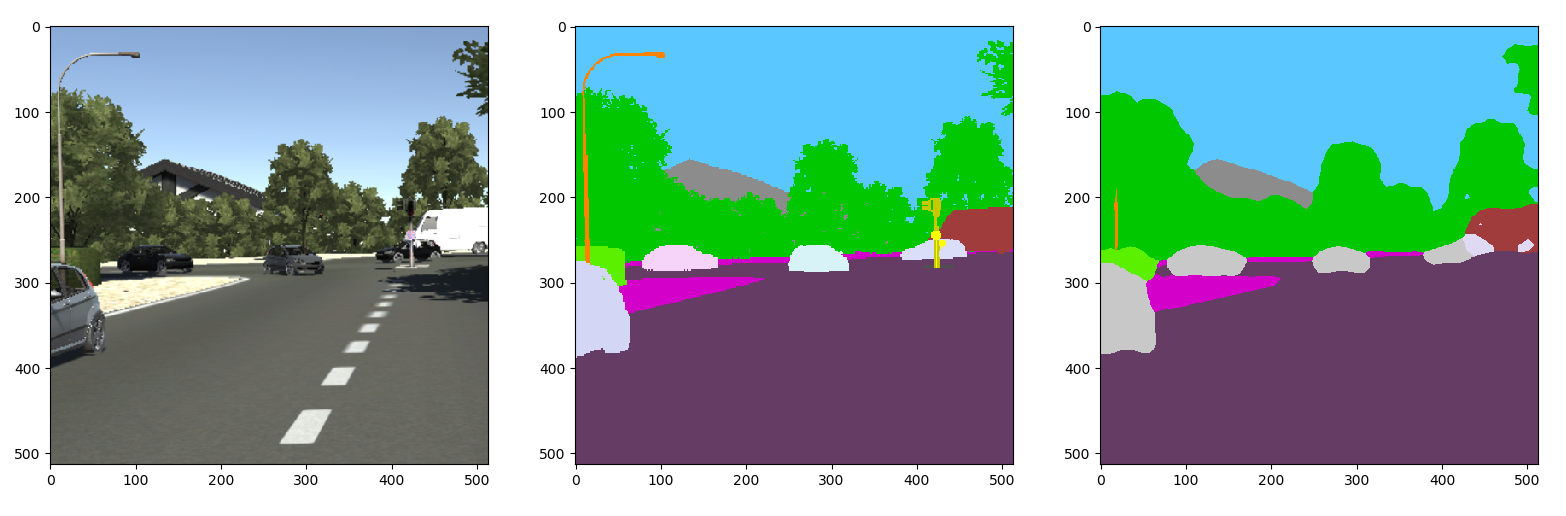
\includegraphics[width=0.9\textwidth]{./graphics/coarse_details.png}
   \caption{Initial segmentation result. Sample \texttt{0001/clone/00340}.}
   \label{fig:coarse_details}
\end{figure}

I initially thought this is because of i) the lower maximum resolution of
input images (375px vs the recommended 513px) and ii) the fewer number of
optimization steps in the first batch of experiments. While addressing i)
improved the things a bit, IoU didn't increase significantly. Currently
waiting for results on $60k$ optimization steps vs 30k as trained until now.

\textbf{My current hypothesis is that the \texttt{output\_stride}, the ratio
between input and output spatial resolutions is too high right now, impeding
the model from learning fine details. I'll give some details below on how I
plan to address this.}

\subsection{Training setup}
\label{sub:training_setup}

The latest training setup which we will build on is described here:
\begin{enumerate}
   \item Model definition \url{https://pytorch.org/hub/pytorch_vision_deeplabv3_resnet101/}
   \item Pre-trained \texttt{ResNet-101} backbone.
   \item Polynomial learning rate schedule $(1 - \frac{step}{total\_steps})^{\alpha}$
   \item The \texttt{output\_stride} (ratio of input to output) is 16. In
   \cite{chen2017rethinking} this is 16 for the first 30k optimization steps
   then changed to 8 for the final 30k steps in order to increase the
   resolution of the feature maps. See the paper for details.
   \item Augmentation:
      \begin{itemize}
         \item \texttt{RandomScale} to min=1.4, max=2.0
         \item \texttt{RandomCrop} of size 513px
         \item \texttt{RandomHorizontalFlip}
      \end{itemize}
   \item Images are normalized with the ImageNet statistics.
   \item BatchNorm layers are trained during the entire run. The Pascal-VOC
   protocol trained these layers for the first 30k steps only.
   \item This configuration allows for batches of size 10.
\end{enumerate}

\subsection{Further steps}
\label{sub:further_steps}

\begin{enumerate}
   \item Start using the Real Kitti validation split and report the IoU.
   \item Experiment with training \texttt{output\_stride} of 8. This has the
   disadvantage of decreasing the batch size enough to mess with the
   \texttt{BatchNorm} layers. I am considering doing this:
   \begin{enumerate}
      \item Train 30k iterations with \texttt{output\_stride=16,
      batch\_size=10} and tuning \texttt{BatchNorm}
      \item Set \texttt{output\_stride=8} and freeze \texttt{BatchNorm}, thus
      mirroring the protocol in the original paper.
   \item Adjust the protocol to make the comparison possible with
   \cite{chen2018learning}
   \end{enumerate}
   \item Start evaluating with \texttt{output\_stride=8}, even if trained at
   a smaller resolution.
\end{enumerate}

% bib stuff
\clearpage
\nocite{*}
\printbibliography
\addtocontents{toc}{\protect\vspace{\beforebibskip}}
\addcontentsline{toc}{section}{\refname}
\end{document}
